% !TEX root = ../main.tex
\section{Marco teórico y ejercicios resueltos}

\subsection{Comparación de complejidades teóricas}
En la Tabla \ref{tab:complejidad_teorica} comparamos los costos asintóticos entre un BST estándar, un Splay Tree de diccionario y un Link-Cut Forest sobre caminos dinámicos.

\begin{table}[H]
    \caption{Comparación de complejidad temporal entre estructuras}
    \label{tab:complejidad_teorica}
    \centering
    \footnotesize
    \begin{tabular*}{\textwidth}{@{\extracolsep{\fill}}lccc}
        \toprule
        \textbf{Operación} & \textbf{BST Estándar} & \textbf{Splay Tree} & \textbf{Link-Cut Forest} \\
        \midrule
        Búsqueda / Consulta & $O(n)$ peor caso & $O(\log n)$ amortizado & $O(\log n)$ amortizado (\texttt{find\_root}) \\
        Inserción / Enlace  & $O(n)$ peor caso & $O(\log n)$ amortizado & $O(\log n)$ amortizado (\texttt{link}) \\
        Eliminación / Corte & $O(n)$ peor caso & $O(\log n)$ amortizado & $O(\log n)$ amortizado (\texttt{cut}) \\
        Suma sobre camino   & $O(n)$ recorrido & No aplica & $O(\log n)$ amortizado (\texttt{path\_sum}) \\
        Cambio de raíz      & No aplica        & No aplica & $O(\log n)$ amortizado (\texttt{make\_root}) \\
        \bottomrule
    \end{tabular*}
\end{table}

\subsection{Ejercicio resuelto 1: rotaciones e instrumentación de \texttt{splay}}
Evaluamos el caso \textit{zig-zig} sobre la cadena $100 \leftarrow 50 \leftarrow 20$. Al invocar \texttt{splay(20)}, primero rota el padre $50$ sobre $100$, y luego $20$ sobre $50$, aplanando el árbol y dejando a $20$ en la raíz:

\begin{lstlisting}[language=Python, caption={Código central de rotaciones y splay (Resuelto 1)}, label={lst:resuelto_1}]
def _rotate(self, x):
    p = x.parent; beta = x.right if p.left is x else x.left
    self._replace_parent_link(p, x)
    if p.left is x: x.right, p.left = p, beta
    else:           x.left, p.right = p, beta
    p.parent = x; self.stats.rotations += 1
    if beta: beta.parent = p

def splay(self, x):
    while x.parent:
        p, g = x.parent, x.parent.parent
        if not g: self.stats.zig += 1; self._rotate(x)
        elif (g.left is p) == (p.left is x):
            self.stats.zig_zig += 1; self._rotate(p); self._rotate(x)
        else: self.stats.zig_zag += 1; self._rotate(x); self._rotate(x)
\end{lstlisting}

\begin{lstlisting}[style=consolestyle, caption={Salida de consola del Ejercicio Resuelto 1}]
Arbol: 100 <- 50 <- 20 | In-order: [20, 50, 100] -> splay(20) -> Raiz: 20 | In-order: [20, 50, 100] (Rot=2, Zig-zig=1)
\end{lstlisting}

\begin{figure}[H]
    \centering
    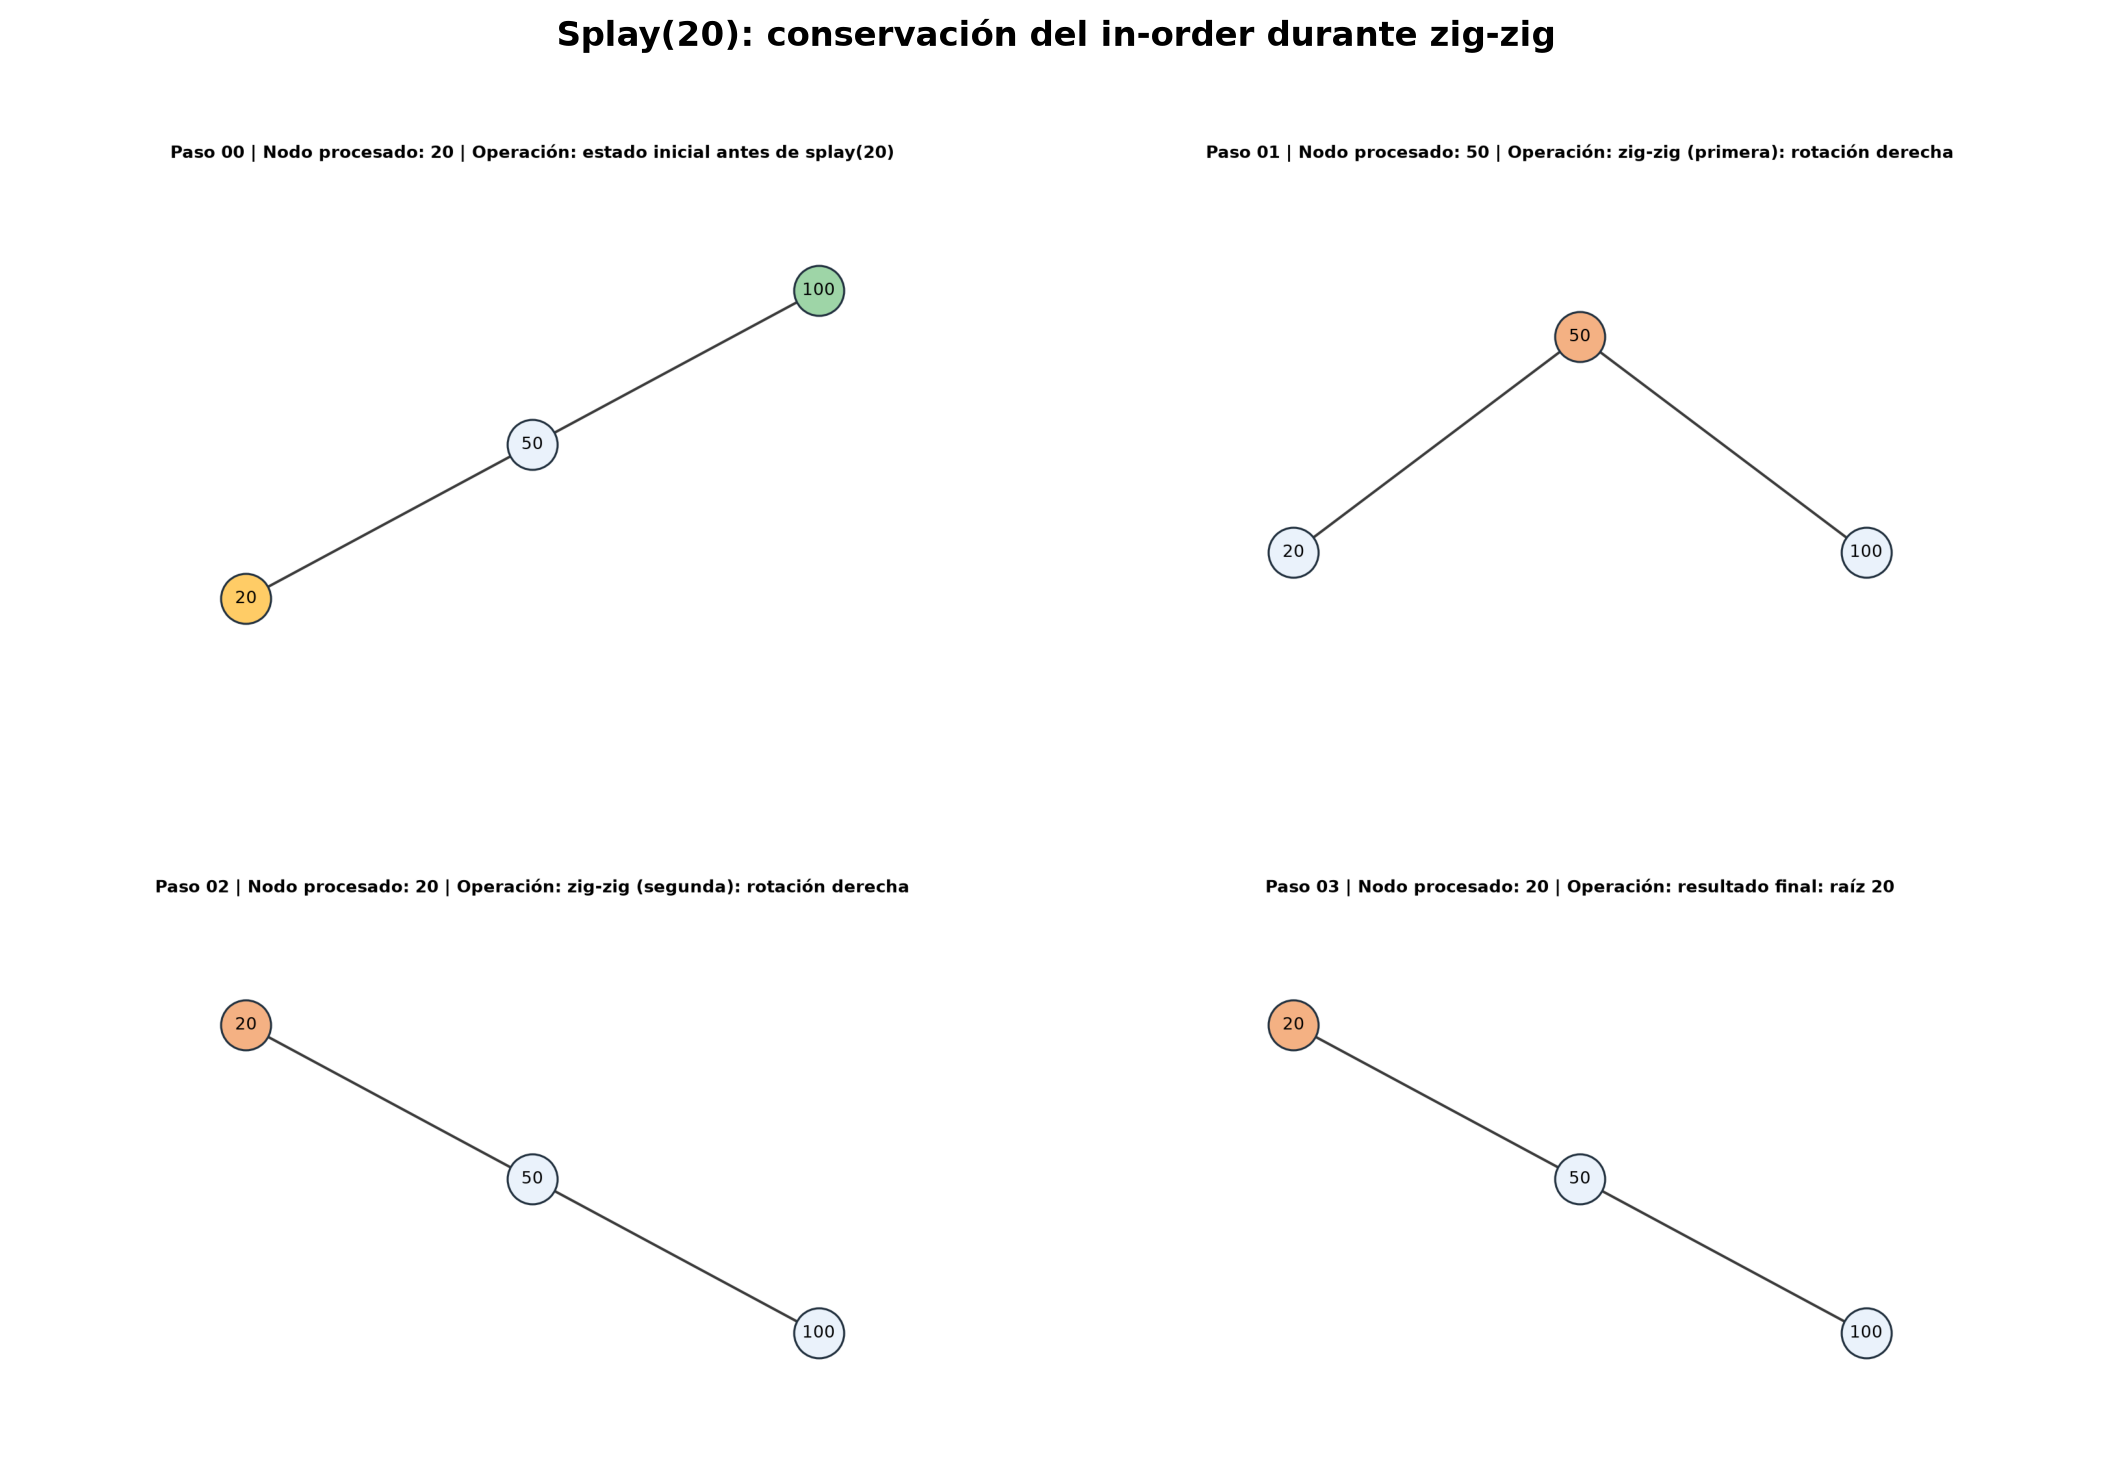
\includegraphics[width=\textwidth, keepaspectratio]{fig_splay_rotaciones_resumen.png}
    \caption{Paso a paso de las rotaciones durante el caso zig-zig de \texttt{splay(20)}}
    \label{fig:splay_rotaciones}
\end{figure}

% -------------------------------------------------------------------------
\subsection{Ejercicio resuelto 2: búsqueda, inserción y eliminación}
Comprobamos las operaciones de diccionario insertando la secuencia $[40, 20, 60, 10, 30, 50, 70]$. La búsqueda de $30$ la eleva a la raíz, la búsqueda fallida de $25$ aproxima al último nodo visitado ($30$), y la eliminación de $40$ separa los subárboles unificándolos mediante \texttt{join}.

\begin{lstlisting}[style=consolestyle, caption={Salida de consola del Ejercicio Resuelto 2}]
Insert [40, 20, 60, 10, 30, 50, 70] -> Raiz: 70 | search(30): Raiz=30 | search(25): Raiz=30 | delete(40): True
\end{lstlisting}

\begin{figure}[H]
    \centering
    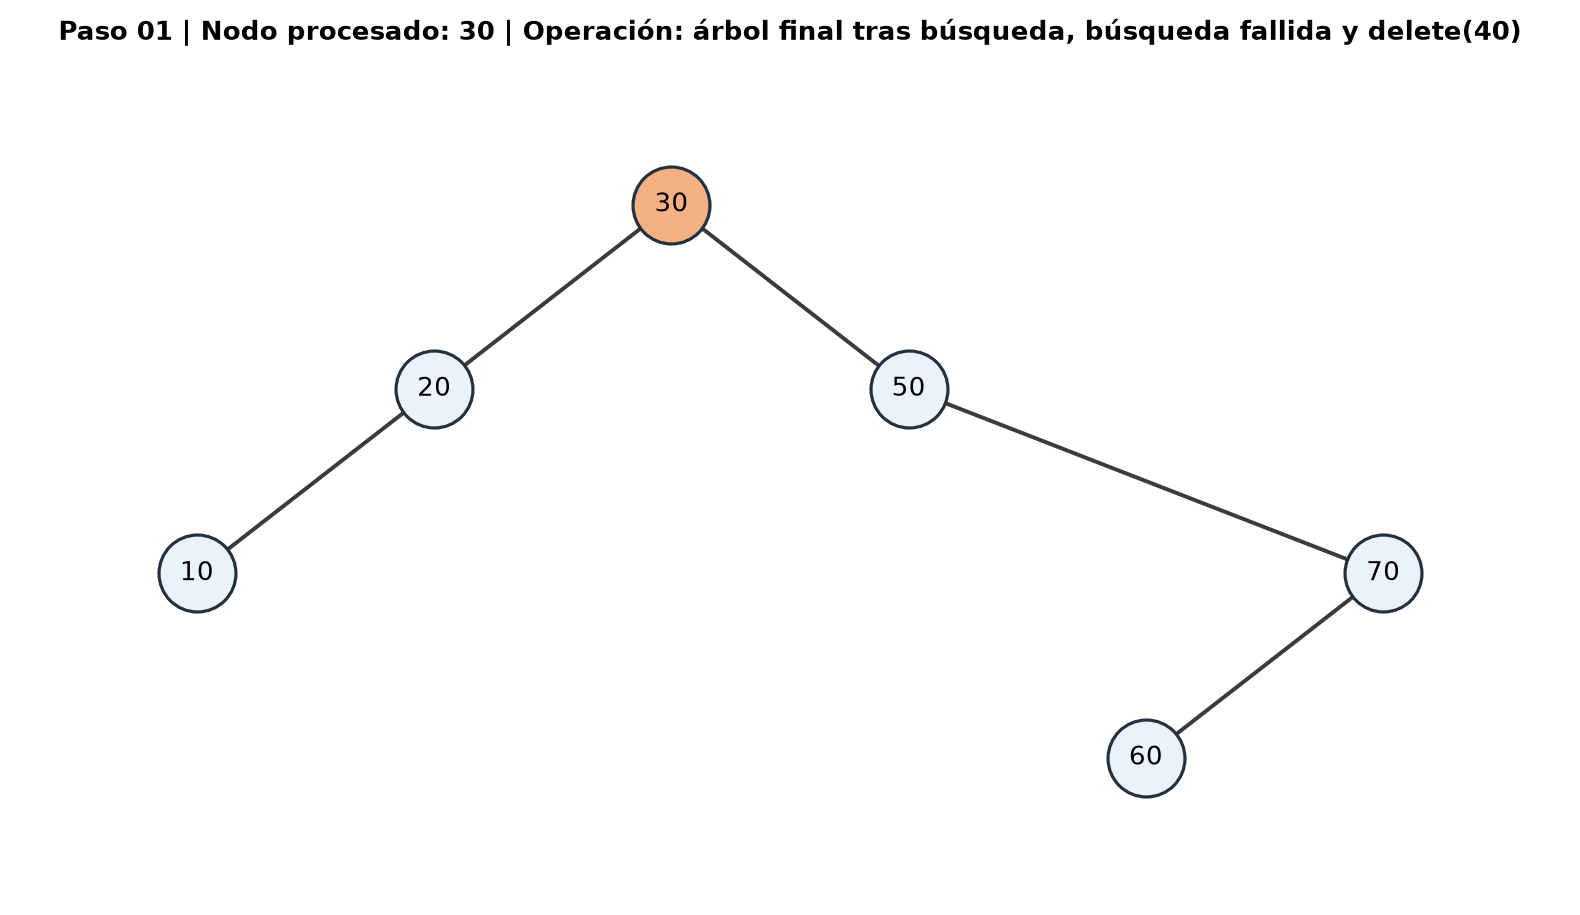
\includegraphics[width=0.95\textwidth, height=0.34\textheight, keepaspectratio]{fig_splay_operaciones_final.png}
    \caption{Estructura final del Splay Tree tras completar las operaciones de diccionario}
    \label{fig:splay_operaciones_final}
\end{figure}

\subsection{Ejercicio resuelto 3: bosque de referencia con BFS}
Para validar el Link-Cut Tree, construimos un modelo simple basado en listas de adyacencia y búsqueda en anchura (BFS). En la prueba oficial evaluamos los vértices $\{1: 4, 2: 7, 3: 2, 4: 9, 5: 1, 6: 6, 7: 3\}$ con aristas $\{(1, 2), (1, 3), (2, 4), (2, 5), (3, 6), (3, 7)\}$:

\begin{lstlisting}[style=consolestyle, caption={Salida de consola de la prueba del bosque de referencia}]
Aristas: [(1, 2), (1, 3), (2, 4), (2, 5), (3, 6), (3, 7)] | Camino(4, 6): [4, 2, 1, 3, 6] -> Suma=28 | cut(1, 3) -> connected(4, 6): False
\end{lstlisting}
Este oráculo permite auditar automáticamente las pruebas diferenciales aleatorias del bosque dinámico.
